\documentclass[../differential_geometry.tex]{subfiles}
\begin{document}
\section{Aula 02 - de Fevereiro, 2026}
\subsection{Motivações}
\begin{itemize}
	\item Curvas Parametrizadas em \(\mathbb{R}^{n}\);
	\item Mudança de Parâmetro.
\end{itemize}
\subsection{Curvas Parametrizadas}
É possível ver o espaço \(\mathbb{R}^{n}\) de duas maneiras: um espaço vetorial de dimensão n munido do limite de um produto escalar (bilinear):
\[
	\langle \omega , \eta  \rangle = \sum\limits_{i=1}^{n}\omega_{i}\eta_{i} = \omega_1\eta_1 + \dotsc +\omega_{n}\eta_{n},
\]
onde \(\omega = (\omega_1, \dotsc , \omega_{n})\) e \(\eta = (\eta_1, \dotsc , \eta_{n})\), sendo que \(\langle \omega , \eta  \rangle = 0\) se, e somente se, \(\omega = 0\) ou \(\eta =0\);
a outra forma, por outro lado, consiste em enxergar \(\mathbb{R}^{n}\) como um conjunto de pontos determinados a partir de um certo ponto chamado origem, usada para obter os outros a partir de coordenadas que usam ela como referência, ou seja, é uma abordagem que usa uma noção da \textbf{distância euclidiana} -- a partir de dois pontos A e B, pode-se formar um vetor \(\vec{AB}\) e definir
\[
	d(A, B) = \sqrt[]{\langle \vec{AB}, \vec{AB} \rangle}.
\]
O problema é que essa construção é bem teórica, e para fazer contas, precisamos escolher um sistema de coordenadas para utilizar; neste caso, utilizaremos o sistema \((O, E)\), onde E é a base canônica de \(\mathbb{R}^{n}\) como espaço vetorial, de forma que podemos escrever
\[
	A = (a_1, \dotsc , a_{n}) \Longleftrightarrow \vec{OA} = (a_1,\dotsc ,a_{n})_{E},\quad B = (b_1,\dotsc ,b_{n})\Longleftrightarrow \vec{OB} = (b_1,\dotsc ,b_{n})_{E}
\]
e, consequentemente,
\[
	\vec{AB} = (b_{1}-a_{1}, \dotsc b_{n}-a_{n})_{E},
\]
a partir de onde damos a definição explícita da distância:
\[
	d(A, B)= \sqrt[]{(b_1-a_1)^{2}+\dotsc + (b_{n}-a_{n})^{2}}.
\]

Finalmente, podemos definir uma curva propriamente:
\begin{def*}
	Uma \textbf{curva em \(\mathbb{R}^{n}\)} é uma reta deformada, ou seja, a partir de um intervalo I de \(\mathbb{R}\), mapeamos seus pontos em \(\mathbb{R}^{n}\) com uma aplicação específica.
	Logo, definimos ela como uma aplicação \(\alpha :I\subseteq \mathbb{R}\rightarrow \mathbb{R}^{n}\) suave (de classe \(\mathcal{C}^{\infty}\))\footnote{As coordenadas de \(\alpha \) são todas funções infinitamente diferenciáveis.} e I é um intervalo aberto de \(\mathbb{R}\). \(\square\)
\end{def*}
\begin{def*}
	A imagem \(\alpha (I)\) é chamada de \textbf{traço da curva} em \(\mathbb{R}^{n}\), e \(\alpha \) é chamada \textbf{parametrização do traço da curva}.
	O ponto onde \(\alpha \) está sendo aplicada é chamado \textbf{parâmetro da curva}, de forma que escrevemos
	\[
		\alpha (u)=(\alpha_1(u), \dotsc , \alpha_{n}(u)),
	\]
	sendo \(\alpha_{i}:I\rightarrow \mathbb{R}\) funções infinitamente diferenciáveis. \(\square\)
\end{def*}

\begin{tcolorbox}[
		skin=enhanced,
		title=Observação,
		fonttitle=\bfseries,
		colframe=black,
		colbacktitle=cyan!75!white,
		colback=cyan!15,
		colbacklower=black,
		coltitle=black,
		drop fuzzy shadow,
		%drop large lifted shadow
	]
	O intervalo na definição acima \textit{pode} ser fechado, mas requer que a pessoa defina as derivadas à esquerda e à direita de uma função.

	Além disso, em geral, podemos omitir a menção do traço toda vez, sendo necessária apenas quando necessário: ao falar apenas da curva, falamos do traço da curva, e ao falar do traço, estamos falando especificamente daquela parametrização em específico.
\end{tcolorbox}

\begin{figure}[H]
	\begin{center}
		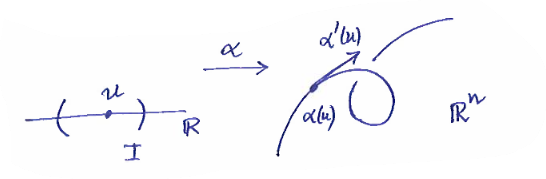
\includegraphics[height=0.7\textheight, width=0.7\textwidth, keepaspectratio]{./Images/parametrized_curve_02.png}
	\end{center}
	\caption{Uma curva \(\alpha \) mapeando um intervalo aberto I em uma curva de \(\mathbb{R}^{n}\).}
\end{figure}

\begin{def*}
	O vetor \(\alpha'(u) = (\alpha_{1}'(u), \dotsc , \alpha_{n}'(u))\) é chamado \textbf{vetor tangente à curva no ponto u ou \(\alpha (u)\)}, também conhecido como \textbf{velocidade}. \(\square\)
\end{def*}
\begin{def*}
	Uma curva \(\alpha \) é dita \textbf{regular em u} se a vetor tangente à curva em u é diferente de zero, isto é, se \(\alpha'(u)\neq 0\); por outro lado, se o vetor tangente \(\alpha '(u)\) nunca se anula, ou seja, \(\alpha'(u)\neq 0\) para todo u em I, então diremos apenas que a curva \(\alpha \) é \textbf{regular}; caso contrário, se \(\alpha (u)=0\) para algum u em I, falaremos que \(\alpha \) é \textbf{singular no ponto u}. \(\square\)
\end{def*}
\begin{def*}
	Se \(\alpha \) é uma curva regular, então o \textbf{vetor tangente unitário} à \(\alpha \) no ponto u é dado por
	\[
		t(u) = \frac{\alpha '(u)}{\Vert \alpha'(u) \Vert}. \; \square
	\]
\end{def*}
\begin{example}[Círculo]
	Uma curva em \(\mathbb{R}^{2}\) é, por exemplo, \(\alpha :\mathbb{R}\rightarrow \mathbb{R}^{2} \) dada por
	\[
		\alpha (u) = (\cos^{}{u}, \sin^{}{u});
	\]
	da mesma forma, poderíamos definir uma curva implicitamente como o zero de uma função
	\begin{align*}
		f: & \mathbb{R}^{2}\rightarrow \mathbb{R}     \\
		   & (x, y)\longmapsto f(x, y)=x^{2}+y^{2}-1,
	\end{align*}
	tal que
	\[
		\alpha (\mathbb{R})=f^{-1}(0).
	\]
	Além disso, essa curva é regular!
\end{example}
\begin{example}[Hélice]
	Defina \(\alpha :\mathbb{R}\rightarrow \mathbb{R}^{3}\) por
	\[
		\alpha (u) = (\cos^{}{u}, \sin^{}{u}, u),
	\]
	formando uma curva suave e regular, pois
	\[
		\alpha '(u) = (-\sin^{}{u}, \cos^{}{u}, 1) \neq (0,0,0).
	\]

	Observe que \(x^{2}(u)+y^{2}(u)=1\), que permite concluirmos que o traço da curva \(\alpha \) é contido no cilindro em \(\mathbb{R}^{3}\) de equação \(x^{2}+y^{2}=1\):
	\begin{figure}[H]
		\begin{center}
			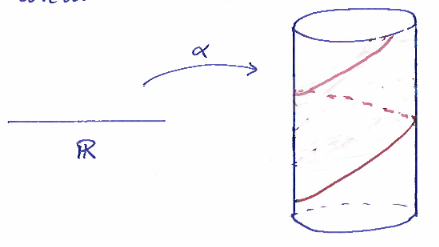
\includegraphics[height=0.5\textheight, width=0.5\textwidth, keepaspectratio]{./Images/helix_02.png}
		\end{center}
		\caption{A curva é resultado de mapear a reta em uma hélice!}
	\end{figure}
\end{example}
\begin{example}[Cúspide]
	O próximo exemplo de curva é uma suave que possui uma singularidade na origem -- a curva cúspide, definida por
	\begin{align*}
		\alpha : & \mathbb{R}\rightarrow\mathbb{R}^{2}     \\
		         & u\longmapsto \alpha (u)=(u^{3}, u^{2}),
	\end{align*}
	com velocidade no ponto u dada como \(\alpha '(u) = (3u^{2}, 2u)\), ou seja, \(\alpha '(0) = (0,0)\).
	\begin{figure}[H]
		\begin{center}
			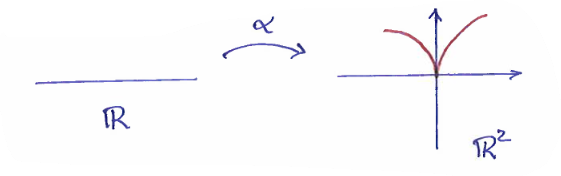
\includegraphics[height=0.5\textheight, width=0.5\textwidth, keepaspectratio]{./Images/cuspid_02.png}
		\end{center}
		\caption{Imagem da cúspide}
	\end{figure}
\end{example}
\begin{example}[Nó]
	Nossa próxima curva é o primeiro exemplo de um nó, e vamos usar ele para mostrar como se esboça uma curva sem usar tecnologia! Defina
	\begin{align*}
		\alpha : & \mathbb{R}\rightarrow\mathbb{R}^{2}         \\
		         & u\longmapsto \alpha (u)=(u^{3}-u, u^{2}-1),
	\end{align*}
	satisfazendo regularidade e suavidade:
	\[
		\alpha '(u)=(3u-1, 2u)\neq (0,0),\quad \forall u\in \mathbb{R}.
	\]

	Para esboçar o traço de \(\alpha \), vamos estudar suas funções componentes
	\begin{align*}
		 & x(u)=u^{3}-u  \\
		 & y(u)=u^{2}-1.
	\end{align*}
	Sobre elas, temos as derivadas e pontos de inflexão
	\begin{align*}
		 & x'(u)=3u^{2}-1,\; x'(u)=0 \Longleftrightarrow u = \pm \frac{\sqrt[]{3}}{3} \\
		 & y'(u)=2u,\; y'(u)=0 \Longleftrightarrow u = 0.
	\end{align*}
	Nos pontos de \(\alpha \) aplicada ao zero da derivada da função \(x(u)\), ou seja, em \(\alpha \bigl(\frac{\sqrt[]{3}}{3}\bigr)\), o vetor tangente é vertical; por outro lado, no ponto \(\alpha (0)\), o vetor tangente é horizontal! Isso já permite encontrarmos alguns dos pontos importantes para \(\alpha \), mas não todos.

	O passo seguinte consiste em procurar os pontos de auto-interseção, ou seja, os pontos onde \(\alpha (u_1)=\alpha (u_2)\) para \(u_1\neq u_2\); podemos fazer isso igualando as duas funções que definem a curva e resolvendo o sistema resultante:
	\begin{align*}
		 & u_{1}^{2}-1 = u_{2}^{2}-1 \stackrel{u_2\neq u_1}\Rightarrow u_{2}=-u_{1}                                        \\
		 & u_{1}^{3}-u_{1} = u_{2}^{3}-u_{1} \Longleftrightarrow u_{1}^{3}-u_1 = 0 \Longleftrightarrow u_1(u_{1}^{2}-1)=0,
	\end{align*}
	ou seja, \(u_1 = \pm1\), pois caso contrário, se fosse 0, os pontos seriam iguais.

	Consequentemente, temos um único ponto de auto-interseção em \(\alpha (1)=\alpha (-1)=(0,0)\).
	\begin{figure}[H]
		\begin{center}
			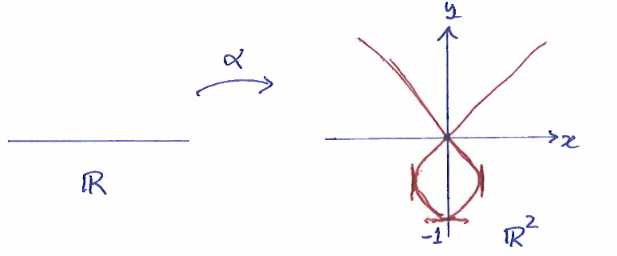
\includegraphics[height=\textheight, width=\textwidth, keepaspectratio]{./Images/node_02.png}
		\end{center}
		\caption{as linhas representam as tangentes, e dá pra visualiza como é um ponto de auto-interseção.}
	\end{figure}

\end{example}
\begin{example}[Gráfico de uma Função]
	Seja \(f:I\subseteq \mathbb{R}\rightarrow \mathbb{R}\) uma função suave e \(\alpha:I\rightarrow \mathbb{R}^{2}\) a curva dada por
	\[
		\alpha (u)=(u, f(u)).
	\]
	O gráfico da função f é o traço de \(\alpha \).
\end{example}
\begin{prop*}
	O gráfico de uma função suave é uma curva regular.
\end{prop*}
\begin{proof*}
	Seja \(f:I\subseteq \mathbb{R}\rightarrow \mathbb{R}\) uma função suave e \(\alpha:I\rightarrow \mathbb{R}^{2}\) a curva dada por
	\[
		\alpha (u)=(u, f(u)).
	\]
	Então,
	\[
		\alpha'(u)=(1, f'(u)) \neq (0,0)
	\]
	para qualquer ponto u em \(\mathbb{R}.\) \qedsymbol
\end{proof*}

\subsection{Mudança de Parâmetros}
Considere a estrada Washington Luiz, representada por uma curva em \(\mathbb{R}^{3}\); ela em si é fixa, mas pode ser o traço de vários moivmentos de carros! Por exemplo, um carro A pode percorrê-lo em 120 minutos entre São Carlos e Campinas, e um carro B faria a mesma rota em 90 minutos.
Estes diferentes casos podem ser representados por duas curvas \(\alpha_{A}:[0,120]\rightarrow \mathbb{R}^{3}\) e \(\alpha_{B}:[0,90]\rightarrow \mathbb{R}^{3}\), representando os movimentos dos dois carros, e teremos \(\alpha_{A}\neq \alpha_{B}\); no entanto, os traços de ambas representam o trecho da rodovia entre as duas cidades, ou seja, \(\alpha_{A}([0,120])=\alpha_{B}([0,90])\)! O que mudou, então?

Nosso interesse está no traço de uma curva \(\alpha \), e existem infinitas maneiras de \textit{parametrizar} este traço, resultando em ``rotas'' diferentes para a mesma curva.
\begin{def*}
	Seja C uma curva em \(\mathbb{R}^{n}\). Uma \textbf{parametrização de C} é uma aplicação \(\alpha :I\subseteq \mathbb{R}\rightarrow \mathbb{R}^{n}\) tal que \(\alpha (I)=C.\; \square\)
\end{def*}
A ideia dessa definição é que uma parametrização de uma curva é exatamente o caso de percorrer a mesma curva de formas diferentes, por exemplo os carros A e B do exemplo anterior, e essa forma diferente está codificada na mudança do intervalo de onde a curva sai.
\begin{example}
	O círculo unitário em \(\mathbb{R}^{2}\) pode ser parametrizado por
	\[
		\alpha (s)=(\cos^{}{s}, \sin^{}{s}), \;s\in [0,2\pi ],
	\]
	ou ainda por
	\[
		\beta (u)=\biggl(\cos^{}{\frac{u}{2}}, \sin^{}{\frac{u}{2}}\biggr),\; s\in [0, 4\pi ].
	\]
	Ambas traçam o mesmo círculo, apesar dos intervalos diferentes! Mais ainda, podemos traduzir de uma curva para outra -- basta definirmos a função
	\begin{align*}
		h: & [0, 4\pi ]\rightarrow[0,2\pi ] \\
		   & u\longmapsto h(u)=\frac{u}{2},
	\end{align*}
	tal que
	\[
		\beta (u)=\alpha (h(u)).
	\]

	Em termos de um diagrama, isso equivale a
	\begin{center}
		\begin{tikzpicture}[
				observed/.style = {rectangle, thick, text centered, draw, text width = 6em},
				latent/.style = {ellipse, thick, draw, text centered, text width = 6em},
				error/.style ={circle, thick, draw, text centered},
				confounding/.style = {rectangle, thick, text centered, draw, text width = 6em, minimum width = 5.5in},
				outcome/.style = {rectangle, thick, draw, text centered, minimum height = 3.5in, text width = 6em},
			]

			\node(T) at (0,1){\([0, 2\pi ]\)};
			\node(BL) at (0,-1){\([0, 4\pi ]\)};
			\node(BR) at (2,1){\(\mathbb{R}^{2}\)};

			\draw[Arrow](T)--node[midway, above] {\(\alpha \)}(BR);
			\draw[Arrow](BL)--node[midway, left] {h}(T);
			\draw[Arrow](BL)--node[midway, below] {\(\beta \)}(BR);

		\end{tikzpicture}
	\end{center}
\end{example}

Motivados pelo exemplo prévio, definimos:
\begin{def*}
	Seja \(\alpha :I \rightarrow \mathbb{R}^{n}\) uma curva suave e regular. Uma \textbf{mudança de parâmetros para \(\alpha \)} é uma função \(h:J\rightarrow I\), onde J é um intervalo aberto de \(\mathbb{R}\), tal que:
	\begin{itemize}
		\item[i)] h é suave;
		\item[ii)] a derivada de h nunca se anula: \(h'(t)\neq 0\) para todo t em J; e
		\item[iii)] h é sobrejetora: \(h(J)=I\).
	\end{itemize}
	\begin{center}
		\begin{tikzpicture}[
				observed/.style = {rectangle, thick, text centered, draw, text width = 6em},
				latent/.style = {ellipse, thick, draw, text centered, text width = 6em},
				error/.style ={circle, thick, draw, text centered},
				confounding/.style = {rectangle, thick, text centered, draw, text width = 6em, minimum width = 5.5in},
				outcome/.style = {rectangle, thick, draw, text centered, minimum height = 3.5in, text width = 6em},
			]

			\node(T) at (0,1){I};
			\node(BL) at (0,-1){J};
			\node(BR) at (2,1){\(\mathbb{R}^{2}\)};

			\draw[Arrow](T)--node[midway, above] {\(\alpha \)}(BR);
			\draw[Arrow](BL)--node[midway, left] {h}(T);
			\draw[Arrow](BL)--node[midway, right] {\(\beta = \alpha \circ h \)}(BR);

		\end{tikzpicture}
	\end{center}

	A aplicação \(\beta :J\rightarrow \mathbb{R}^{n}\) dada por \(\beta (t)=\alpha (h(t))\) é chamada \textbf{reparametrização} da curva \(\alpha. \; \square\)

\end{def*}
\begin{tcolorbox}[
		skin=enhanced,
		title=Observação,
		fonttitle=\bfseries,
		colframe=black,
		colbacktitle=cyan!75!white,
		colback=cyan!15,
		colbacklower=black,
		coltitle=black,
		drop fuzzy shadow,
		%drop large lifted shadow
	]
	O traço de \(\alpha \) e de \(\beta \) na definição de reparametrização é o mesmo! Afinal,
	\[
		\alpha (h(I)) = \beta (J).
	\]
\end{tcolorbox}

Uma das formas de parametrização mais comuns é utilizando o \textit{comprimento de arco}: tome uma curva qualquer em \(\mathbb{R}^{3}\); queremos parametrizar essa curva de alguma forma e medir seu comprimento sem retirar partes dela, mas como fazer isso? Ora, sabemos calcular o comprimento dos segmentos de reta, então podemos copiar algumas ideias do cálculo integral e escrever a curva como um monte de segmentos de retas:
\begin{figure}[H]
	\begin{center}
		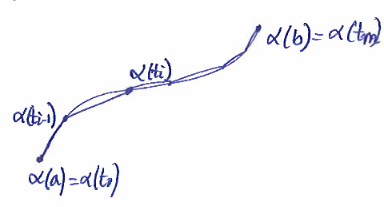
\includegraphics[height=0.5\textheight, width=0.5\textwidth, keepaspectratio]{./Images/arc_length_03.png}
	\end{center}
\end{figure}
Assim, quanto maior a quantidade de segmentos de retas, melhor será a aproximação! Logo, faz sentido definirmos a noção seguinte:
\begin{def*}
	Seja \(\alpha :I\rightarrow \mathbb{R}^{n}\) uma curva suave e regular, e seja \([a, b]\subseteq I\) um subintervalo de I. Tomando a partição
	\[
		\mathcal{P}: a=t_{0}<t_1<\dotsc <t_{m}=b
	\]
	do intervalo \([a, b]\), com \(\Vert \mathcal{P} \Vert = \max\limits_{i}\Delta_{i} = | t_{i}-t_{i-1} |.\)

	Definimos o \textbf{comprimento de arco da curva} \(\alpha \) entre \(\alpha (a)\) e \(\alpha (b)\) como sendo
	\[
		\Vert \alpha '(t) \Vert=\mathrm{Arco}(\alpha ) \coloneqq \lim_{\Vert \mathcal{P} \Vert\to 0} \sum\limits_{i=1}^{m}\Vert \alpha (t_i)-\alpha (t_{i-1}) \Vert. \; \square
	\]
\end{def*}
A notação como a norma da velocidade é justificada -- denotemos por \(\Delta \ell_{i}\) a diferença
\[
	\Delta \ell_{i} = \Vert \alpha (t_{i})-\alpha (t_{i-1}) \Vert = \sqrt[]{(\Delta x_1)^{2}+(\Delta x_2)^{2} + \dotsc + (\Delta x_{n})^{2}},
\]
onde \((\Delta x_1, \dotsc , \Delta x_n)\) são as coordenadas do vetor \((\alpha(t_{i})-\alpha (t_{i-1}))\). Agora, vamos escolher uma partição regular, com \(\Delta t_{i} \) sendo a mesma para todos os pontos da partição, digamos
\[
	\Delta t_{i} = t_{i}-t_{i-1} = \Delta t = \frac{b-a}{m};
\]
então, segue que
\[
	\frac{\Delta \ell_{i}}{\Delta t} = \sqrt[]{\biggl(\frac{\Delta x_1}{\Delta t}\biggr)^{2} + \biggl(\frac{\Delta x_2}{\Delta t}\biggr)^{2} + \dotsc + \biggl(\frac{\Delta x_n}{\Delta t}\biggr)^{2}}.
\]
Logo, quando \(\Delta t\) tende a zero, obtemos
\[
	\frac{\mathrm{d}\ell }{\mathrm{d}t} = \sqrt[]{\biggl(\frac{\mathrm{d}x_1}{\mathrm{d}t}\biggr)^{2} + \biggl(\frac{\mathrm{d}x_2}{\mathrm{d}t}\biggr)^{2} + \dotsc + \biggl(\frac{\mathrm{d}x_n}{\mathrm{d}t}\biggr)^{2}} = \Vert \alpha '(t) \Vert.
\]

Portanto, definimos a versão entre pontos quaisquer do comprimento de arco da curva:
\begin{def*}
	O \textbf{comprimento de arco de uma curve entre dois pontos \(t_{0}\) e \(t\)} é definido por
	\[
		\ell (t) = \int_{t_{0}}^{t}\Vert \alpha '(u) \Vert \mathrm{d}u.\; \square
	\]
\end{def*}
\begin{tcolorbox}[
		skin=enhanced,
		title=Observação,
		fonttitle=\bfseries,
		colframe=black,
		colbacktitle=cyan!75!white,
		colback=cyan!15,
		colbacklower=black,
		coltitle=black,
		drop fuzzy shadow,
		%drop large lifted shadow
	]
	Caso aconteça de \(\Vert \alpha '(s) \Vert=1\) para todo ponto s no intervalo I, então
	\[
		\ell (s)=\int_{s_{0}}^{s} \mathrm{d}u = s-s_{0},
	\]
	onde, neste caso, o parâmetro s é o comprimento de arco da curva, a menos da constante \(s_{0}!\)
\end{tcolorbox}
\begin{def*}
	Se \(\Vert \alpha '(s) \Vert=1\) para todo ponto s em I, dizemos que a curva é \textbf{parametrizada pelo comprimento de arco.} \(\square\)
\end{def*}
\begin{prop*}
	Seja \(\alpha :I\rightarrow \mathbb{R}^{n}\) uma curva suave e regular; então, a parametrização
	\[
		\beta = \alpha \circ \ell^{-1}:J\rightarrow \mathbb{R}^{n}
	\]
	é sempre uma parametrização da curva pelo comprimento de arco, com \(J = \ell (I).\)
\end{prop*}
\begin{proof*}
	Seja
	\[
		\ell (t) = \int_{t_{0}}^{t}\Vert \alpha'(u) \Vert \mathrm{d}u,
	\]
	sendo \(t_{0}\) um ponto fixo em I.
	Note que \(| \ell (t) |\) mede o comprimento da curva \(\alpha \) entre os pontos \(\alpha (t)\) e \(\alpha (t_{0})\), mesmo se \(t\) não for maior que \(t_{0}\).
	Vamos mostrar que a função \(\ell :I\rightarrow \ell (I)=J\) tem uma inversa.

	De fato, a derivada \(\ell '(t) = \Vert \alpha '(t) \Vert \) é sempre positiva, garantindo a existência de \(\ell ^{-1}\) e a suavidade; assim, derivando \(\beta (s)\) conforme dado no enunciado da proposição, obtemos
	\begin{align*}
		\beta '(s) = \alpha '(\ell^{-1}(s)) \cdot (\ell^{-1}(s))' & = \alpha '(\ell ^{-1}(s))\frac{1}{\ell'(\ell^{-1}(s))}              \\
		                                                          & = \frac{\alpha'(\ell^{-1}(s))}{\Vert \alpha '(\ell ^{-1}(s)) \Vert} \\
		                                                          & \Rightarrow \Vert \beta '(s) \Vert =1.
	\end{align*}
	Portanto, \(\beta \) é parametrizada pelo comprimento de arco. \qedsymbol
\end{proof*}
\begin{tcolorbox}[
		skin=enhanced,
		title=Observação,
		fonttitle=\bfseries,
		colframe=black,
		colbacktitle=cyan!75!white,
		colback=cyan!15,
		colbacklower=black,
		coltitle=black,
		drop fuzzy shadow,
		%drop large lifted shadow
	]
	A parametrização pelo comprimento de arco é muito importante para estabelecer resultados teóricos, mas ela é meio inútil na prática; por exemplo, a catenária é dada por
	\[
		\alpha (u) = (u, \cosh^{}{u}),\quad u\in \mathbb{R},
	\]
	donde temos \(\alpha '(u) = (1, \sinh^{}{u})\), ou seja,
	\[
		\Vert \alpha '(u) \Vert^{2} = 1 + \sinh^{2}{u} = \cosh^{2}{u}.
	\]
	Portanto, \(\alpha \) não é parametrizada pelo comprimento de arco.
	Caso fossemos fazer essa parametrização, teríamos
	\[
		\ell (t) = \int_{0}^{t}\Vert  \alpha '(t)\Vert \mathrm{d}t = \sinh^{}{t} \quad\&\quad  \ell^{-1}(t) = \sinh^{-1}{t} = \ln^{}{(t+\sqrt[]{t^{2}+1})};
	\]
	logo,
	\[
		\beta (s)=(\ln^{}{(s+\sqrt[]{s^{2}+1})}, \cosh^{}{(\ln^{}{(s+\sqrt[]{s^{2}+1})})}),
	\]
	que realmente não é muito interessante pra fazermos contas.
\end{tcolorbox}
\end{document}
